\documentclass[12pt]{article}

\usepackage[a4paper,margin=1in]{geometry}
\usepackage{fontspec}
\usepackage{titlesec}
\usepackage{longtable}
\usepackage{array}
\usepackage{xcolor}
\usepackage{colortbl}
\usepackage{fancyhdr}
\usepackage{hyperref}
\usepackage{enumitem}
\usepackage{booktabs}
\usepackage{amssymb}
\usepackage{graphicx}
\usepackage{caption}
\usepackage{setspace}
\usepackage{verbatim}
\usepackage{float}
\graphicspath{{report_screenshots/}}
\captionsetup{font=small, labelfont=bf, skip=4pt}
\setlength{\intextsep}{6pt}
\setlength{\textfloatsep}{8pt}

\definecolor{navy}{HTML}{1F3864}
\definecolor{linegray}{HTML}{999999}
\definecolor{tablehead}{HTML}{1F3864}

\titleformat{\section}{\normalfont\Large\bfseries}{\thesection}{0.6em}{}
\titleformat{\subsection}{\normalfont\large\bfseries}{\thesubsection}{0.6em}{}

\pagestyle{fancy}
\setlength{\headheight}{14pt}
\fancyhf{}
\fancyhead[R]{\small\itshape Internet Programming Lab -- Project Report}
\fancyfoot[C]{\thepage}
\renewcommand{\headrulewidth}{0.4pt}

\newcolumntype{L}[1]{>{\raggedright\arraybackslash}p{#1}}

\hypersetup{colorlinks=true, urlcolor=navy, linkcolor=black, citecolor=navy}

\setstretch{1.15}

\title{}
\date{}

\begin{document}

% ================= COVER PAGE =================
\begin{titlepage}
\centering
\vspace*{1.2cm}
{\bfseries\large CSE 4113 -- Internet Programming Lab}\\[1.8cm]
{\bfseries\Huge Project Report}\\[1.8cm]

{\bfseries\Large Digital Knowledge Platform (DKP)}\\[0.3cm]
{\itshape\color{gray} Semicolon Squad}\\[1.4cm]

{\bfseries Submitted By}\\[0.5cm]

\renewcommand{\arraystretch}{1.4}
\begin{tabular}{|L{7cm}|L{5cm}|}
\hline
\rowcolor{tablehead} \textcolor{white}{\bfseries Team Member} & \textcolor{white}{\bfseries Student ID} \\
\hline
Yuki Bhuiyan & 2021816226 \\
\hline
Faria Yasmin & 2021611197 \\
\hline
Hasibul Islam Sifat & 2021211218 \\
\hline
Md. Nuruzzaman & 2021611232 \\
\hline
\end{tabular}

\vspace{1.4cm}
{\bfseries 28th Batch}\\
Department of Computer Science \& Engineering\\
University of Dhaka\\[1cm]

{\bfseries Submitted On}\\
{25 July 2026}
\vfill

\end{titlepage}

% ================= PROJECT LINKS =================
\section*{Project Links}
\addcontentsline{toc}{section}{Project Links}

\renewcommand{\arraystretch}{1.4}
\begin{longtable}{|L{5cm}|L{9.5cm}|}
\hline
\rowcolor{tablehead} \textcolor{white}{\bfseries Item} & \textcolor{white}{\bfseries URL} \\
\hline
Public Git Repository (main2 branch) & \url{https://github.com/Semicolon-Squad-DU/Digital_Knowledge_platform/tree/main2} \\
\hline
Deployed Application URL & \url{https://semicolon.farefin.com/} -- self-hosted via Docker Compose behind an Nginx reverse proxy handling TLS termination (see Section 9.2 for the storage-endpoint fix this required). \\
\hline
API Docs (Swagger/Postman) & \texttt{docs/openapi.yaml} in the repository (OpenAPI 3.0) \\
\hline
Demo Video & \url{https://www.youtube.com/watch?v=qHFxDeTWKLI} \\
\hline
\end{longtable}

\bigskip
\tableofcontents
\newpage

% ================= SECTION 1 =================
\section{Introduction}

\subsection{Problem Definition and Context}
Universities and research organizations generally maintain their digital archives, library catalogs, research records, and student project data through separate, unconnected systems. This fragmentation makes it difficult for students, faculty, and staff to locate and share institutional knowledge efficiently. The Digital Knowledge Platform (DKP) was built to address this by consolidating four traditionally separate institutional functions -- a digital archive, a library circulation system, a research output repository, and a student project showcase -- into one role-based web application, backed by a single PostgreSQL database, so that every user group works from a consistent and permission-controlled view of the same institutional data.

\subsection{Target Users and Use Cases}
The platform defines seven distinct roles, arranged in an explicit hierarchy from least to most privileged: \textbf{guest}, \textbf{member}, \textbf{student\_author} and \textbf{researcher} (equal privilege level), \textbf{archivist} and \textbf{librarian} (equal privilege level), and \textbf{admin}.

\begin{itemize}[leftmargin=1.4em]
\item \textbf{Guests} (unauthenticated visitors) can browse only public-tier content -- published archive items, the public library catalog, and public showcase projects.
\item \textbf{Members} are the base authenticated role: they can borrow and return library items, join wishlists and holds, comment and react on content, and RSVP to events.
\item \textbf{Student Authors} additionally submit and manage their own showcase projects for advisor review.
\item \textbf{Researchers} additionally publish and retract their own research outputs, create research labs, and act as project advisors who approve or request changes on showcase submissions assigned to them.
\item \textbf{Archivists} manage the full lifecycle of the digital archive -- uploading, editing, versioning, publishing, and archiving documents -- and review access requests for restricted material.
\item \textbf{Librarians} run the library circulation desk: issuing and returning books, managing holds and fines, and operating the barcode scanner workflow.
\item \textbf{Admins} have full platform oversight: user and role management, audit log review, system configuration, backups, and content moderation.
\end{itemize}

\subsection{Core Features}
\begin{itemize}[leftmargin=1.4em]
\item \textbf{Digital Archive} -- tiered-access document repository with a formal draft/review/published/archived lifecycle, full version history, and an access-request workflow for restricted material.
\item \textbf{Library Management} -- catalog browsing, issue/return with automatic fine calculation, a first-come-first-served hold queue, renewals, wishlists, and barcode-based circulation.
\item \textbf{Research Repository} -- output records organized under research labs, with one-click citation export in BibTeX, APA, and MLA formats.
\item \textbf{Student Project Showcase} -- project submission with an advisor-driven review workflow (pending review, published, or changes requested) and a public project gallery.
\item \textbf{Community Features} -- threaded comments with moderation and an ``accepted answer'' mechanism, four-type reactions, and events with seat-limited RSVP and automatic waitlist promotion.
\item \textbf{Notifications} -- a per-user notification feed with configurable preferences, separate from admin-authored, role-targeted announcements.
\item \textbf{Administration and Security} -- role-based access control across seven roles, an immutable audit log, scheduled encrypted backups, and a fail-closed malware-scanning upload pipeline.
\end{itemize}

\subsection{Tech Stack Overview}
\renewcommand{\arraystretch}{1.3}
\begin{longtable}{|L{2.8cm}|L{4.2cm}|L{6.5cm}|}
\hline
\rowcolor{tablehead} \textcolor{white}{\bfseries Layer} & \textcolor{white}{\bfseries Technology} & \textcolor{white}{\bfseries Justification} \\
\hline
Frontend & Next.js 14 (App Router), TypeScript & File-based routing and a server/client component split, with type safety across a multi-role interface. \\
\hline
Styling & Tailwind CSS & Fast, consistent utility-first styling across nineteen top-level routes and many feature modules. \\
\hline
State Management & Zustand, TanStack Query v5 & Zustand handles lightweight local UI state; TanStack Query manages server-state caching and synchronization with the API. \\
\hline
Forms and Validation & React Hook Form, Zod & Type-safe schema validation shared between the form layer and the API. \\
\hline
Backend & Node.js, Express, TypeScript & A lightweight REST framework suited to a modular, feature-based API with per-role route guards. \\
\hline
Database & PostgreSQL 16 & Relational integrity for cross-referenced institutional records (e.g. a research output linked to its auto-generated archive entry), with schema changes tracked through 29 explicit, numbered SQL migrations. \\
\hline
Search & Elasticsearch 8.12 & Provisioned to power full-text archive search, though currently disabled at runtime with an automatic fallback to PostgreSQL \texttt{ILIKE} search (see Section 2.4). \\
\hline
Cache & Redis 7 & Fast, ephemeral storage for caching and rate-limiting. \\
\hline
File Storage & MinIO (S3-compatible) & Self-hosted object storage with server-side AES-256 encryption for uploaded files and backups. \\
\hline
Authentication & JWT, Google Sign-In & Stateless access/refresh token authentication, with Google Sign-In as an alternative login method verified directly against Google's endpoints. \\
\hline
Hosting & Docker Compose & Runs Postgres, Redis, Elasticsearch, ClamAV, MinIO, and the application containers together under a single, reproducible setup. \\
\hline
\end{longtable}

Third-party services used include Google Sign-In for authentication, MailHog for email testing in development, and ClamAV for scanning every uploaded file before it is stored.

% ================= SECTION 2 =================
\section{System Architecture}

\subsection{High-Level Architecture Diagram}
The system follows a three-tier architecture: a Next.js frontend communicates with an Express REST API over \texttt{/api}, which in turn reads and writes to PostgreSQL, with Redis, Elasticsearch, and MinIO acting as supporting services for caching, search, and file storage respectively.

\begin{figure}[H]
\centering
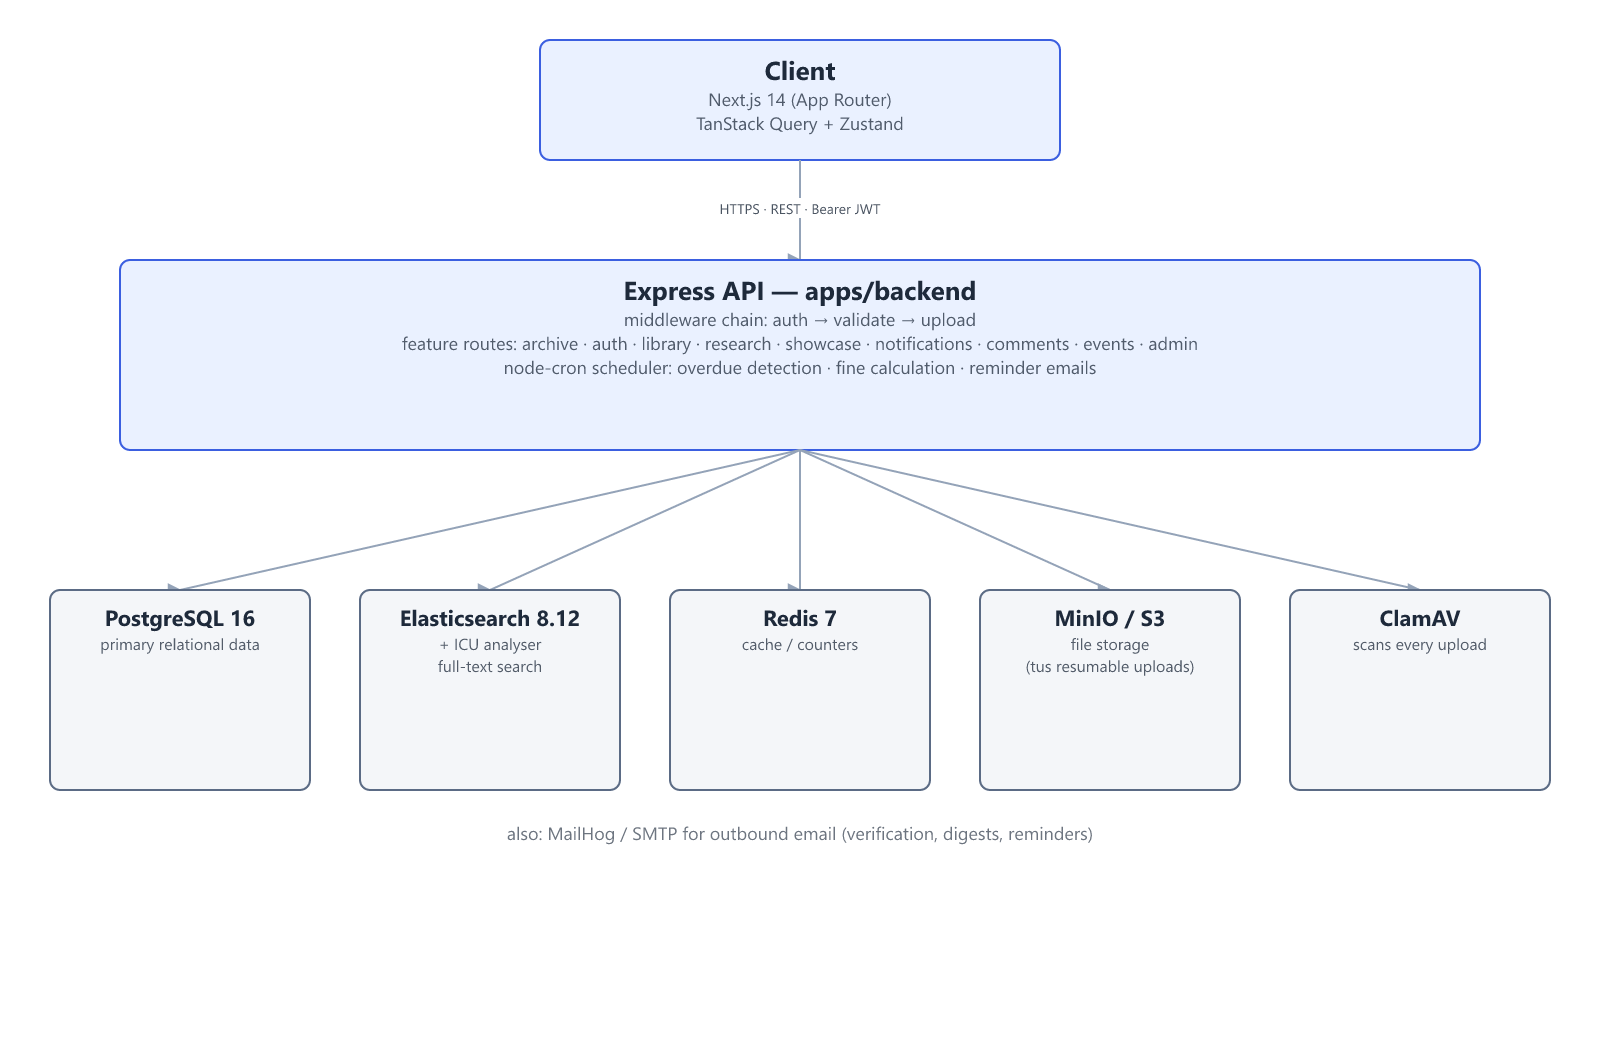
\includegraphics[width=0.95\linewidth]{architecture-diagram.png}
\caption{High-level architecture: the frontend never talks to Postgres, Elasticsearch, Redis, or MinIO directly -- every request goes through the Express API.}
\end{figure}

\subsection{Frontend Architecture}
The frontend is built with the Next.js 14 App Router. Source code is organized under \texttt{apps/frontend/src}: the \texttt{app/} directory holds route segments, \texttt{features/} holds domain-specific modules that mirror the backend's feature structure, \texttt{components/ui/} holds shared UI primitives, \texttt{store/} holds Zustand state, and \texttt{lib/} holds shared utilities and API clients. Server state is managed through TanStack Query, while local UI state is managed through Zustand. Forms are built with React Hook Form and validated with Zod. The application exposes nineteen top-level routes: \texttt{about}, \texttt{admin}, \texttt{archive}, \texttt{contact}, \texttt{dashboard}, \texttt{events}, \texttt{forgot-password}, \texttt{librarian}, \texttt{library}, \texttt{login}, \texttt{notifications}, \texttt{privacy}, \texttt{profile}, \texttt{register}, \texttt{repository}, \texttt{research}, \texttt{search}, \texttt{showcase}, and \texttt{terms}, alongside the home page and shared layout.

\subsection{Backend Architecture}
The backend is built with Express and TypeScript, organized under \texttt{apps/backend/src} into: \texttt{core/} for configuration, the database pool, and middleware (including authentication, role-based access control, and entity-level access rules); \texttt{features/} with one folder per domain -- archive, auth, library, research, showcase, notifications, comments, reactions, events, and admin -- each containing its own routes and controllers; \texttt{infrastructure/} for the S3/MinIO client, the backup service, the email service, the antivirus scanner, and the Elasticsearch client; \texttt{jobs/} for scheduled cron tasks; and \texttt{routes/} for route aggregation. This feature-based layout keeps each domain's routing, business logic, and access rules together rather than splitting them across generic MVC layers.

\subsection{Database Design}
The database schema is defined in \texttt{init.sql} and extended through 29 incremental, numbered SQL migrations located in \texttt{apps/backend/src/core/db/migrations/}. Migrations are applied with \texttt{npm run db:migrate}. No ORM is used; all queries go through a raw \texttt{pg} connection pool, which gives direct control over indexing, transactional row-locking (used in the borrowing and event-RSVP workflows), and query structure for the search-heavy tables.

The schema is organized around the following core entities:

\begin{itemize}[leftmargin=1.4em]
\item \textbf{users} -- accounts, with one of seven roles (guest, member, student\_author, researcher, archivist, librarian, admin), membership status, and Google OAuth fields.
\item \textbf{archive\_items}, \textbf{archive\_item\_tags}, \textbf{archive\_versions}, \textbf{tags} -- the digital archive, including full version history and tag-based categorization.
\item \textbf{access\_requests} -- the approval workflow for archive and research items above a viewer's access tier.
\item \textbf{labs}, \textbf{lab\_members}, \textbf{research\_outputs} -- the research repository, organized under research labs with a designated head researcher.
\item \textbf{student\_projects} -- the project showcase, including an assigned advisor and review comments.
\item \textbf{catalog\_items}, \textbf{borrows}, \textbf{hold\_requests}, \textbf{wishlists}, \textbf{fines} -- the library lending module, including an auto-generated barcode per item.
\item \textbf{notifications}, \textbf{notification\_preferences}, \textbf{announcements} -- the in-app notification system, separating individual system notifications from admin-authored broadcasts.
\item \textbf{comments}, \textbf{comment\_moderation} -- threaded, self-referencing community discussion, added in migration 005.
\item \textbf{audit\_logs} -- an append-only log of state-changing events; \texttt{UPDATE} and \texttt{DELETE} on this table are blocked at the database level with a \texttt{CREATE RULE} statement, so audit history cannot be altered even by an administrator with direct database access.
\item \textbf{refresh\_tokens}, \textbf{system\_configs}, \textbf{backups} -- authentication session state and platform administration data.
\end{itemize}

\begin{figure}[H]
\centering

\includegraphics[width=0.95\linewidth]{er-diagram.png}
\caption{Core entities grouped by module. Every module's tables carry a foreign key back to \texttt{users} (\texttt{uploaded\_by}, \texttt{borrower\_id}, \texttt{advisor\_id}, etc.); the dashed edges show the auto-archive-entry relationship described in Section 4.1.}
\end{figure}

\paragraph{Data Synchronization.} The platform does not use WebSockets or Server-Sent Events. Live-feeling updates are achieved through polling with TanStack Query: the notification feed refetches from the server automatically every 30 seconds, so a user sees new notifications without manually refreshing the page. All other data is fetched on navigation and on-demand through standard TanStack Query cache invalidation after a mutation, such as submitting a form or approving a request.

% ================= SECTION 3 =================
\section{API Documentation}

\subsection{API Design Overview}
The backend exposes a REST API, with all routes prefixed under \texttt{/api}. There is currently no explicit API versioning scheme in place. A health-check endpoint is available at \texttt{GET /health}.

\subsection{Endpoint Reference}
\renewcommand{\arraystretch}{1.3}
\begin{longtable}{|L{1.4cm}|L{3.4cm}|L{6.3cm}|L{2.3cm}|}
\hline
\rowcolor{tablehead} \textcolor{white}{\bfseries Method} & \textcolor{white}{\bfseries Route} & \textcolor{white}{\bfseries Description} & \textcolor{white}{\bfseries Auth} \\
\hline
POST & /api/auth/register & Create a new user account & No \\
\hline
POST & /api/auth/login & Authenticate and receive access/refresh tokens & No \\
\hline
POST & /api/auth/refresh & Exchange a refresh token for a new access token & No \\
\hline
POST & /api/auth/logout & Invalidate the current session & Yes \\
\hline
GET & /api/auth/me & Retrieve the current authenticated user & Yes \\
\hline
* & /api/archive/* & Upload, tagging, versioning, status transitions, and tiered search & Yes (tiered) \\
\hline
* & /api/library/* & Catalog, barcode lookup, issue/return/renew, fines, holds, wishlist & Yes (role-based) \\
\hline
* & /api/research/* & Research outputs, citation export, labs & Yes \\
\hline
* & /api/showcase/* & Student project submission, advisor review, gallery & Mixed \\
\hline
* & /api/comments/*, /api/reactions/* & Threaded comments, moderation, reactions & Mixed \\
\hline
* & /api/events/* & Events, seat-limited RSVP with waitlisting & Mixed \\
\hline
* & /api/notifications/* & Notification feed, preferences, admin announcements & Yes \\
\hline
* & /api/admin/* & User/role management, audit logs, backups, system config & Yes (Admin) \\
\hline
GET & /health & Service health check & No \\
\hline
\end{longtable}

\subsection{Swagger / Postman Collection Link}
An OpenAPI 3.0 specification covering the endpoint surface listed in Section 3.2 is included in the repository at \texttt{docs/openapi.yaml}. It documents each route's method, parameters, authentication requirement, and expected responses at a summary level; request/response schemas for the lower-traffic routes are intentionally left brief and can be filled in from the corresponding \texttt{*.routes.ts} handler as time permits. The file can be pasted directly into the Swagger Editor (\url{https://editor.swagger.io}) or imported into Postman to generate an interactive collection.

\subsection{Sample Request and Response}
The following illustrates \texttt{POST /api/auth/login}.

\textbf{Request:}
\begin{verbatim}
POST /api/auth/login
Content-Type: application/json

{
  "email": "researcher@dkp.edu.bd",
  "password": "Test@123456"
}
\end{verbatim}

\textbf{Response (200 OK):}
\begin{verbatim}
{
  "success": true,
  "data": {
    "access_token": "<jwt>",
    "refresh_token": "<jwt>",
    "user": {
      "user_id": "...",
      "name": "Researcher User",
      "email": "researcher@dkp.edu.bd",
      "role": "researcher",
      "membership_status": "active",
      "department": "...",
      "avatar_url": null
    }
  }
}
\end{verbatim}

The password hash is explicitly stripped from the response before it is sent to the client. On invalid credentials, the API responds with HTTP 401 and a generic message (``Invalid email or password''), rather than indicating whether the email or the password was incorrect, to avoid account enumeration.

% ================= SECTION 4 =================
\section{Core Modules -- Detailed Behavior}

This section describes the business logic of each major module in enough detail to distinguish it from a generic CRUD implementation.

\subsection{Digital Archive}
Every archive item carries one of four access tiers: \texttt{public}, \texttt{member}, \texttt{staff}, and \texttt{restricted}. Each role is mapped to the set of tiers it can view: guests see only \texttt{public}; members and student authors see \texttt{public} and \texttt{member}; researchers and librarians additionally see \texttt{staff}; archivists and admins see all four, including \texttt{restricted}. An item above a viewer's tier can still be requested through the access-request workflow, and only an approved request grants that specific user access.

Items move through a strict four-state lifecycle -- \texttt{draft} $\rightarrow$ \texttt{review} $\rightarrow$ \texttt{published} $\rightarrow$ \texttt{archived} -- enforced as an explicit state machine rather than a free-form status field. Forward transitions may be performed by archivists, librarians, or admins; moving an item \emph{backward} in the lifecycle (for example, un-publishing a document) is restricted to archivists and admins only. Every document also has full version history: each new file uploaded against an existing item is stored as a new row with an incrementing version number and a snapshot of the metadata at that point in time, so past versions remain retrievable even after the current file is replaced.

Full-text search is designed around Elasticsearch -- a \texttt{multi\_match} query across title, description, authors, and tags, filtered by the caller's allowed access tiers and publish status -- but Elasticsearch is currently disabled at application startup in this deployment, and every search transparently falls back to a PostgreSQL \texttt{ILIKE} query against the same fields. This keeps search functional in the current environment while leaving the Elasticsearch integration in place for when it is enabled.

Research outputs and showcase projects that get published each automatically create a linked, published archive entry, which is how the same document can be discovered both from its origin module (Research or Showcase) and from the general Archive browser.

\subsection{Library Management}
Issuing an item runs through an ordered set of checks: available copies must be greater than zero, the borrower's membership must be active, the borrower must be under the platform's maximum active-borrow limit, and the borrower's outstanding fines must not exceed a fixed threshold. The default loan period is 14 days, the per-user borrow limit is 5 active items, and each loan may be renewed up to 2 times -- renewal is blocked if the item is already overdue or if another member has a pending hold on the same title. Returning an item recalculates its fine at the rate of 5 currency units per day overdue, and automatically promotes the oldest pending hold on that title, if one exists, notifying that member that the item is now available.

Holds are strictly first-come-first-served: fulfilling a hold is blocked if an earlier hold on the same catalog item is still pending or available, not merely by insertion order but by an explicit query comparing request timestamps. Wishlists, by contrast, are a simple personal save-list with no queue or approval step. Every catalog item has an auto-generated barcode, and the issue, return, and lookup endpoints all accept a scanned barcode as an alternative to typing in an item ID, supporting a physical circulation-desk workflow. Bulk catalog import and export is also supported via CSV/XLSX, with a duplicate-detection preview step before any bulk data is committed.

\subsection{Research Repository}
Research outputs are organized under labs, each with a designated head researcher. A researcher can create, edit, and retract their own outputs and can create new labs; retracting an output hides it from search and browsing while preserving the record itself for audit purposes. Every published output is assigned a DKP identifier in the form \texttt{DKP-<year>-<5-digit-code>}, which anchors its citation record. Citation export is available in three formats -- BibTeX, APA, and MLA -- generated directly by the backend rather than through an external citation library, so the exact reference text is fully under the project's control. A researcher may only publish an output at an access tier their own role is permitted to view, preventing accidental over-restriction of content the researcher themselves would then be unable to see.

\subsection{Student Project Showcase}
A showcase submission moves through three states: \texttt{pending\_review} on submission, then either \texttt{published} once approved or \texttt{changes\_requested} if the advisor asks for revisions -- a project in the latter state can be edited and resubmitted, returning it to \texttt{pending\_review}. Review authority is not open to any researcher, however: only the specific user assigned as a project's advisor (or an admin) may approve it or request changes, enforced by comparing the reviewer's user ID against the project's stored advisor. Submission itself requires up to three files -- the project report, an optional demonstration video, and an optional thumbnail image -- each validated by file type before upload. Approving a submission with a report attached automatically creates a corresponding archive entry, so approved student work becomes discoverable through the general archive as well as the showcase gallery.

\subsection{Community Features}
Comments support unlimited-depth threading through a self-referencing parent relationship, and can be attached to archive items, research outputs, or showcase projects. Administrators can flag or hide any comment, and a separate ``accepted answer'' mechanism lets the owner of the underlying content (or an admin) mark a specific reply as the accepted answer, giving the discussion feature a lightweight Q\&A character beyond simple commentary. Reactions are limited to four fixed types -- like, love, clap, and insightful -- and behave as a toggle: reacting again with the same type removes it. Events use seat-limited RSVP with automatic waitlisting: once available seats reach zero, further RSVPs are accepted but marked as waitlisted rather than rejected, and cancelling a confirmed RSVP automatically promotes the longest-waiting waitlisted attendee into the freed seat.

% ================= SECTION 5 =================
\section{Authentication and Security}

\subsection{Authentication Strategy}
Authentication is implemented with JSON Web Tokens, using short-lived access tokens (15 minutes) and longer-lived refresh tokens (7 days). JWT was chosen over session-based authentication for statelessness across the Express API. Google Sign-In is also supported as an alternative login method, verified directly against Google's token-info endpoints using only a client ID, with no client secret stored on the server.

\subsection{Authorization and Role Management}
Role-based access control spans seven roles arranged in an explicit hierarchy -- guest, member, student\_author/researcher, archivist/librarian, and admin -- with route-level guards restricting sensitive operations (uploads, status changes, catalog management, user administration) to the appropriate role or roles. Authentication middleware validates token integrity and checks that the account status is active or pending approval on every request, and separately enforces a server-side inactivity timeout of 30 minutes, computed entirely within PostgreSQL from a stored last-active timestamp rather than trusted to client or server clocks, to avoid clock-drift bugs.

\subsection{Security Measures}
HTTP security headers and request rate limiting are applied at the API layer. Input is validated using Zod schemas shared between the frontend and backend. Every uploaded file passes through an ordered safety chain before it is stored: a per-user daily quota check (50 files or 200 MB per day), a MIME-type allowlist, a 500 MB size limit, a binary file-signature (``magic byte'') check that catches files whose real content does not match their declared type, and a ClamAV malware scan, before finally being written to S3-compatible storage with explicit AES-256 server-side encryption. The malware scan is a fail-closed control: if the ClamAV service cannot be reached, uploads are rejected outright rather than silently allowed through unscanned.

Passwords must satisfy a minimum-strength policy of at least 8 characters including an uppercase letter, a lowercase letter, a digit, and a special character. Credentials are managed through environment variables and are not hardcoded in the codebase.

\subsection{Known Vulnerabilities and Mitigations}
During development, a role-escalation issue was identified in the registration flow: a user could switch to a different role by re-registering with an email address that already existed on the platform, without proving ownership of the account. This was fixed by requiring password verification before an existing email can be used to change roles.

The backup and recovery system explicitly documents a known limitation: because the platform runs against a single-instance PostgreSQL database rather than a multi-node cluster with a standby replica, automated failover in the event of a database outage is out of scope. Scheduled daily backups, retained for 30 days, mitigate data loss but do not provide automatic failover; restoring from a backup is a manual, admin-triggered action that always takes a fresh safety backup of the current database before overwriting anything.

Institutional single sign-on (SAML or OIDC) was considered but not implemented, since no real university identity provider was available to integrate against during development. Domain-restricted registration combined with Google OAuth sign-in was used as a practical substitute.

% ================= SECTION 6 =================
\section{Testing and Quality Assurance}

\subsection{Testing Strategy}
\begin{itemize}[leftmargin=1.4em]
\item \textbf{Backend:} Unit tests are written with Jest and Supertest, with a separate integration test suite run against a Postgres container in CI.
\item \textbf{Frontend:} Component tests are written with Vitest and React Testing Library.
\item \textbf{End-to-end:} Playwright drives browser-level tests against the full stack and a dedicated test database, separate from the shared development database.
\end{itemize}

\subsection{Test Coverage Summary}
The project's requirements specify a target of 70\% test coverage. As of the most recent measurement, actual coverage sits well below that target: backend coverage is configured with a CI-enforced minimum of 18\% (statements/lines), 12\% (branches), and 16\% (functions), while frontend coverage is configured with a CI-enforced minimum of 5\% (statements/lines), 4\% (branches), and 3\% (functions). These thresholds reflect coverage as actually achieved at the time of writing rather than the original target, and are tracked as an open item for the team to improve before final submission.

\subsection{Bug Tracking and Resolution Log}
Bug fixes are tracked through the commit history rather than a separate issue tracker. Representative examples include:
\begin{itemize}[leftmargin=1.4em]
\item A high-severity authentication issue allowing role escalation without password verification during registration.
\item Enforcement of librarian-only access on library management API endpoints, which had been reachable by other roles.
\item Prevention of RSVP changes on events that had already ended.
\item A duplicate-ISBN submission returning an uncaught server error instead of a validation message.
\item Zero-amount fines being generated incorrectly by the fine calculation job.
\item A non-atomic hold-fulfillment process that could violate first-come-first-served ordering under concurrent requests.
\item Improved handling of secure file downloads and access-tier validation on the archive module.
\item Detection of failed uploads to S3/MinIO during the automated backup process.
\end{itemize}

\subsection{Sample Test Cases}
The end-to-end test suite includes cases covering archive access-tier enforcement, a homepage smoke test, and an unauthenticated library catalog search flow.

% ================= SECTION 7 =================
\section{CI/CD and Deployment}

\subsection{Pipeline Overview}
Continuous integration is configured through GitHub Actions and runs on every push and pull request. The pipeline lints and tests the backend and frontend independently, runs an integration test job against a live Postgres service container with all migrations applied, and rejects commits from automated or bot accounts, since this is an assessed academic project. The pipeline does not currently include an automated deployment step.

\subsection{Environments}
\begin{itemize}[leftmargin=1.4em]
\item \textbf{Development:} local Docker Compose services (Postgres, Redis, Elasticsearch, MinIO, MailHog, ClamAV).
\item \textbf{Test:} a disposable test database used by CI and local end-to-end runs.
\item \textbf{Production:} an extended Docker Compose configuration that adds the backend and frontend application containers on top of the base services, driven entirely by environment variables.
\end{itemize}

\subsection{Deployment Steps}
\begin{enumerate}[leftmargin=1.6em]
\item Copy the example environment file and populate it with real configuration values.
\item Configure Google Sign-In by creating an OAuth client ID and registering the deployment domain.
\item Build and start all services with Docker Compose.
\item Verify the deployment through the backend's health-check endpoint.
\end{enumerate}

\subsection{Hosting Platform and Live URL}
The platform is self-hosted via Docker Compose at \url{https://semicolon.farefin.com/} rather than through a managed cloud hosting provider, with an Nginx reverse proxy in front of the application containers handling TLS termination and routing for the frontend, API, and object-storage domains (confirmed via the \texttt{Server: nginx/1.24.0} response header on the live deployment). Local Docker Compose evaluation remains available as a fallback for grading if the live deployment is temporarily unavailable.

\subsection{Monitoring and Logging}
Backend logging is handled with Winston. MailHog is used to capture and inspect outgoing emails in non-production environments. The audit log itself (see Section 2.4) functions as a permanent, tamper-proof application-level activity log, separate from process-level logging.

\subsection{Backup and Recovery}
An automated job produces a compressed \texttt{pg\_dump} of the entire database, uploads it to S3-compatible storage with server-side encryption, and optionally replicates it to a second storage location for redundancy. Backups older than 30 days are automatically deleted. Restoring from a backup is a deliberate, manual action available only to administrators: the system always creates a fresh safety backup of the current database state before a restore proceeds, and aborts the restore entirely if that safety backup fails, so a bad restore can never destroy data that was not already backed up.

% ================= SECTION 8 =================
\section{Repository and Documentation Quality}

\subsection{Branching Strategy and Commit Conventions}
Development took place primarily on a shared integration branch. Commit messages follow a loose convention, with many prefixed by type (\texttt{feat}, \texttt{fix}, \texttt{refactor}, \texttt{chore}, \texttt{style}). Pull request approval is restricted to human team members, and the CI pipeline rejects commits from bot accounts.

\subsection{README Completeness Checklist}
The repository README includes a project overview and feature list, a full technology stack breakdown, a screenshots section, and a contribution guide.

\subsection{Code Organization and Folder Structure}
The project is organized as an npm workspaces monorepo:
\begin{itemize}[leftmargin=1.4em]
\item \texttt{apps/frontend} -- the Next.js application
\item \texttt{apps/backend} -- the Express API
\item \texttt{packages/shared} -- shared TypeScript types used by both applications
\item \texttt{docker/} -- supporting Docker build configuration
\item \texttt{e2e/} -- Playwright end-to-end tests
\item \texttt{scripts/} -- developer tooling scripts
\end{itemize}

\subsection{Local Setup Instructions}
Local setup instructions, including environment configuration and database seeding, are documented separately in the repository's setup guide.

% ================= SECTION 9 =================
\section{Evaluation and Reflection}

\subsection{Web Performance and Core Web Vitals}
The frontend is configured with Next.js's built-in image optimization pipeline, defined through \texttt{images.remotePatterns} in \texttt{next.config.js} and covering both the local MinIO storage endpoint and Amazon S3, and it is built with the \texttt{standalone} output mode for a minimal production runtime. However, this optimization pipeline is not currently exercised in practice: the codebase does not yet use the \texttt{next/image} component or \texttt{next/dynamic} for code-splitting anywhere in the frontend source, so images are rendered as plain HTML \texttt{img} tags without automatic resizing or lazy loading.

Performance metrics (First Contentful Paint, Largest Contentful Paint, and Total Blocking Time) were not measured during the current evaluation and are left for a follow-up assessment. Running Lighthouse or PageSpeed Insights against the homepage and the archive search page at \url{https://semicolon.farefin.com/} would produce these figures.

\subsection{Challenges and Solutions}
Several technical obstacles surfaced during development and deployment, each requiring a specific fix:

\begin{itemize}[leftmargin=1.4em]
\item MinIO rejected file uploads with a ``KMS not configured for a server side encrypted objects'' error once the backend began sending an explicit \texttt{ServerSideEncryption: AES256} header on every upload. This was resolved by configuring a static single-key KMS backend in the Docker Compose file so that MinIO would honour the SSE-S3 header.
\item ClamAV requires several minutes on first boot to download virus definitions before \texttt{clamd} accepts connections, which was initially failing the container's health check before initialization completed. The health check's \texttt{start\_period} was extended to accommodate this.
\item CI integration tests originally applied only the base schema (\texttt{init.sql}) rather than the full set of incremental migrations, allowing tests to pass against a database that did not match the schema running in any real environment. The CI workflow was updated to replay every migration file in sorted order, matching what a fresh installation would do.
\item The team's shared Supabase-hosted \texttt{users} table carries roughly fifty additional columns managed internally by Supabase Auth (e.g. \texttt{encrypted\_password}, \texttt{is\_super\_admin}) that are not defined in \texttt{init.sql}. Because backend queries name columns explicitly rather than using \texttt{SELECT *}, these extra columns remain invisible at the application layer without requiring any change to Supabase's managed schema.
\item Two independent branches created differently-purposed migration files under the same sequence number before merging; migration numbers are now coordinated across branches before a schema change is started.
\item The largest issue occurred on the production deployment, where PDF previews and downloads stopped resolving for end users. This traced back to the production Docker Compose configuration having hardcoded the object-storage endpoint used to generate file URLs to an internal Docker network hostname (\texttt{minio:9000}), resolvable only from within the Compose network -- backend-to-storage calls succeeded, but any presigned URL handed back to a browser was unreachable from the public internet. A related defect compounded the issue: the backend's file-existence check treated any storage error, including a connectivity failure, identically to a genuinely missing file, surfacing a misleading ``file is missing from storage'' message rather than the real cause. Both defects were corrected in the codebase: the storage endpoint is now configurable via environment variable rather than hardcoded, and the existence check distinguishes a confirmed 404 from other failure modes. The deployment itself was also updated to expose MinIO on its own public subdomain behind the Nginx reverse proxy, proxied at the domain root rather than under a path prefix -- MinIO's presigned URLs are SigV4-signed against the exact request path, so a path prefix would need to be stripped before reaching MinIO, which would change the signed path and break every presigned URL with \texttt{SignatureDoesNotMatch}. \texttt{S3\_ENDPOINT} in production now points at that public storage domain instead of the internal container hostname. The fix was verified end-to-end against the local environment: a presigned URL for a genuinely-stored document now resolves to a valid, complete PDF rather than an unreachable address.
\end{itemize}

\subsection{Limitations and Future Work}
\begin{itemize}[leftmargin=1.4em]
\item Elasticsearch is provisioned and integrated in code but currently disabled at runtime; full-text search runs on a PostgreSQL \texttt{ILIKE} fallback instead, which is functionally correct but less scalable and less relevant-ranked than the intended Elasticsearch query.
\item The REST API has no versioning scheme, which would make future breaking changes harder to roll out without affecting existing clients.
\item An OpenAPI 3.0 specification is provided in \texttt{docs/openapi.yaml}, which can be imported into Swagger UI or Postman; a dedicated hosted Swagger UI is not currently deployed, and request/response schemas for the lower-traffic routes are still light on detail.
\item Real-time updates (e.g., notifications) rely on 30-second polling rather than WebSockets or Server-Sent Events, which is simpler to implement but less immediate and slightly less efficient at scale.
\item Automated database failover is not implemented, since the platform runs against a single PostgreSQL instance without a standby replica.
\item Institutional single sign-on is not implemented; Google OAuth and domain-restricted registration are used instead.
\item Research lab membership can currently only be modified directly in the database; no API endpoint exists to add or remove a lab member.
\item Increasing automated test coverage remains a priority for future development, as it currently sits well below the project's own 70\% target.
\item Image optimization has been configured but is not yet used throughout the frontend.
\end{itemize}

\subsection{Lessons Learned}
A precise, testable requirement proved substantially harder to write than the corresponding implementation code; several bugs found during testing traced back to ambiguity left in the original SRS rather than to implementation error.

Prioritising module scope with MoSCoW was necessary to deliver a working core (Digital Archive and Library Management) within the semester timeline, with the remaining modules layered on once that core was stable, rather than attempting all nine planned modules in parallel from the start.

Designing for Bangla-language support from the outset -- database collation, tokenisation strategy, bilingual metadata fields -- proved to be a materially different exercise than retrofitting it would have been; several early schema decisions would likely have needed to be revisited had bilingual support been deferred to a later sprint.

Setting the CI-enforced coverage threshold to the project's actual, currently-achieved coverage rather than to the eventual 70\% target was a deliberate choice: it keeps the coverage gate meaningful as a regression check in the near term, rather than leaving it permanently failing or disabling it outright, while coverage is incrementally raised toward the target.

The production storage outage described in Section 9.2 also illustrated a broader point worth keeping in mind for future deployments: a configuration value serving two different purposes -- the address a server uses to reach a dependency internally, and the address a client must use to reach the same dependency externally -- needs to be modelled as two separate settings from the start. Conflating the two is an easy mistake to make in a Docker Compose-based deployment and a difficult one to diagnose after the fact, since the server-to-server path continues to work normally while only the externally-facing path is broken.

\subsection{Individual Responsibility}
\renewcommand{\arraystretch}{1.5}
\begin{longtable}{|L{2.1cm}|L{7.4cm}|L{2.4cm}|L{2.4cm}|}
\hline
\rowcolor{tablehead} \textcolor{white}{\bfseries Member} & \textcolor{white}{\bfseries Core Responsibilities and Feature Ownership} & \textcolor{white}{\bfseries Commits} & \textcolor{white}{\bfseries Contribution} \\
\hline
Yuki &
Backend development across the Library, Archive, Auth, Showcase, and Research modules, along with access control logic. Built out the platform landing page, including role-based dashboard redirection and the guest layout, and contributed broadly to page development across Research, Library, Showcase, Archive, Admin, and Login. Also maintained a large share of the CI/testing and Docker configuration. &
117 &
37.6\% \\
\hline
Faria &
Backend development on the Library, Archive, and Research modules, including secure file download and access validation, along with test-coverage improvements for notifications and archive features. Led several homepage and landing-page refactors and contributed to Admin, Library, Archive, the Librarian dashboard, Research, Showcase, and Events pages. &
95 &
31.2\% \\
\hline
Sifat &
Backend development on Auth, Library, and Archive modules, including an Elasticsearch reindexing utility and role-aware dashboard logic. Authored the project's initial frontend scaffold, including the first version of the landing page, and later led a full homepage redesign. Also implemented the complete authentication-flow UI, including OTP verification, password reset, and role-based login redirects. &
91 &
18.6\% \\
\hline
Nur &
Frontend-focused contributions centered on the Library module, including the librarian and member dashboard redesign, barcode scanner integration, and catalog UI enhancements. Also contributed backend routes for library catalog management. &
10 &
12.6\% \\
\hline
\end{longtable}

Contribution percentages above are estimated from the relative volume of code changes (insertions and deletions) contributed by each member across the project's git history, and are intended as an approximate guide rather than an exact measure of effort, since they do not account for code review, design discussion, or debugging time.

% ================= APPENDIX =================
\newcommand{\shot}[2]{%
\begin{figure}[H]
\centering
\includegraphics[width=0.8\linewidth]{#1}
\vspace{-2pt}
\caption{#2}
\end{figure}%
}

\section*{Appendix -- Screenshots and UI Walkthrough}
\addcontentsline{toc}{section}{Appendix -- Screenshots and UI Walkthrough}

\subsection*{A.1 Public Site and Authentication}
\shot{01-landing-hero.png}{Landing page hero section.}
\shot{02-landing-stats.png}{Landing page sign-in prompt and platform statistics.}
\shot{03-signin.png}{Sign-in page.}
\shot{04-register.png}{Registration page with role selection.}
\shot{22-forgot-password.png}{Forgot password page.}
\shot{23-reset-password.png}{Password reset using an emailed verification code.}

\subsection*{A.2 Dashboard and Core Modules}
\shot{05-dashboard-researcher.png}{Researcher dashboard.}
\shot{06-archive-browse.png}{Digital Archive browsing and filtering.}
\shot{31-archive-document-pdf-preview.png}{Archive document detail page with in-browser PDF preview.}
\shot{24-archive-access-request.png}{Access request flow for a restricted document.}
\shot{07-research-repository.png}{Research Repository listing.}
\shot{30-research-detail-ai-paper.png}{Research output detail page.}
\shot{32-research-detail-arxiv.png}{Research output detail page for an externally published paper.}
\shot{11-research-upload-form.png}{Research output submission form.}
\shot{08-showcase-list.png}{Student Project Showcase listing.}
\shot{26-showcase-project-detail.png}{Showcase project detail page.}

\subsection*{A.3 Library}
\shot{09-library-catalog.png}{Library catalog browsing and filtering.}
\shot{28-library-book-pdf-preview.png}{Library book detail page with an in-browser page-by-page reader.}
\shot{27-librarian-add-book.png}{Librarian view for adding a book to the catalog.}
\shot{13-wishlist.png}{Member wishlist.}

\subsection*{A.4 Community Features}
\shot{10-events.png}{Events and seminars listing.}
\shot{12-notifications.png}{In-app notifications feed.}

\subsection*{A.5 Profile}
\shot{14-profile-dark-theme.png}{User profile page.}
\shot{15-profile-green-theme.png}{User profile page with an alternate theme selected.}

\subsection*{A.6 Admin Panel}
\shot{16-admin-overview.png}{Admin platform overview.}
\shot{17-admin-analytics.png}{Admin analytics dashboard.}
\shot{25-admin-user-management.png}{Admin user management view.}
\shot{18-admin-audit-logs.png}{Admin audit log viewer.}
\shot{19-admin-system-config.png}{Admin system configuration panel.}
\shot{20-admin-backups.png}{Admin backup management.}
\shot{21-admin-announcements.png}{Admin announcement broadcast composer.}

\subsection*{A.7 Static Pages}
\shot{33-about-page.png}{About page.}
\shot{34-contact-team.png}{Contact page.}
\shot{35-privacy-policy.png}{Privacy Policy page.}

\end{document}
